\documentclass[11pt]{article}
\usepackage[margin=1in]{geometry}
\usepackage{enumitem}
\usepackage{hyperref}
\usepackage{graphicx}
\usepackage{array}
\usepackage{multicol}
\usepackage{longtable}
\usepackage{titlesec}
\usepackage{booktabs}
\usepackage{amsmath}
\usepackage{float}
\usepackage{sectsty}
\sectionfont{\fontsize{14}{16}\selectfont}
\subsectionfont{\fontsize{12}{14}\selectfont}


\begin{document}

\begin{center}
    \large \textbf{Sri Sivasubramaniya Nadar College of Engineering, Chennai} \\
    (An autonomous Institution affiliated to Anna University) \\
    \vspace{0.3cm}
\end{center}

\begin{table}[!h]
\renewcommand{\arraystretch}{1.5}
\resizebox{\textwidth}{!}{%
\begin{tabular}{|l|cll|}
\hline
Degree \& Branch     & \multicolumn{1}{c|}{B.E. Computer Science \& Engineering} & \multicolumn{1}{l|}{Semester}        & V                                        \\ \hline
Subject Code \& Name & \multicolumn{3}{c|}{ICS1512 - Machine Learning Algorithms Laboratory}                                                                              \\ \hline
Academic year       & \multicolumn{1}{c|}{2025-2026 (Odd)}                        & \multicolumn{1}{c|}{Batch: 2023-2028} & \multicolumn{1}{c|}{\textbf{Due date: }} \\ \hline
\end{tabular}%
}
\end{table}

\vspace{0.5cm}

\begin{center}
 \textbf{Experiment 3: Email Spam or Ham Classification using Naïve Bayes, KNN, and SVM}
\end{center}

\noindent
\section{Aim:} 
 To classify emails as spam or ham using three classification algorithms — Naïve Bayes, K-Nearest Neighbors (KNN), and Support Vector Machine (SVM)—and evaluate their performance using accuracy metrics and K-Fold cross-validation.

\vspace{0.4cm}
\noindent
\section{Libraries used:}
\begin{itemize}
    \item {Pandas}
    \item {Numpy}
    \item {Matplotlib}
    \item {Scikit-learn}
    \item {Time}
\end{itemize}

\noindent
\section{Objective:} 
The objective of this assignment is to implement and compare the performance of three classification algorithms—Naïve Bayes, K-Nearest Neighbors (KNN), and Support Vector Machine (SVM)—for classifying emails as spam or ham. This includes preprocessing the dataset, training the models using K-Fold cross-validation, and evaluating them based on accuracy metrics.

\section{Code with Plot}
\begin{verbatim}
# TRAINING + EVALUATION CODE OF GIVEN MODEL
def evaluate_model(name, model, X_train, X_test):
    start_time = time.time()
    model.fit(X_train, y_train)
    end_time = time.time()
    y_pred = model.predict(X_test)
    print(f"\n{name} Performance:")
    print(f"Accuracy :  {accuracy_score(y_test, y_pred):.4f}")
    print(f"Precision:  {precision_score(y_test, y_pred, average='macro'):.4f}")
    print(f"Recall   :  {recall_score(y_test, y_pred, average='macro'):.4f}")
    print(f"F1 Score :  {f1_score(y_test, y_pred, average='macro'):.4f}")
    print(f"Training Time: {(end_time - start_time):.4f} seconds")

    fig, axes = plt.subplots(1, 2, figsize=(12, 5))

    cm = confusion_matrix(y_test, y_pred)
    disp = ConfusionMatrixDisplay(confusion_matrix=cm)
    disp.plot(ax=axes[0], cmap='Blues')
    axes[0].set_title('Confusion Matrix')

    y_prob = model.predict_proba(X_test)[:, 1]
    fpr, tpr, _ = roc_curve(y_test, y_prob)
    roc_auc = auc(fpr, tpr)

    axes[1].plot(fpr, tpr, label=f'AUC = {roc_auc:.2f}', color='darkorange')
    axes[1].plot([0, 1], [0, 1], linestyle='--', color='gray')
    axes[1].set_xlabel('False Positive Rate')
    axes[1].set_ylabel('True Positive Rate')
    axes[1].set_title('ROC Curve')
    axes[1].legend()
    axes[1].grid(True)
    plt.tight_layout()
    plt.show()

    
\end{verbatim}

\begin{verbatim}
# NAIVE BAYES - GAUSSIAN
evaluate_model("GaussianNB", GaussianNB(), X_train, X_test)
\end{verbatim}

\begin{figure}[H]
\centering
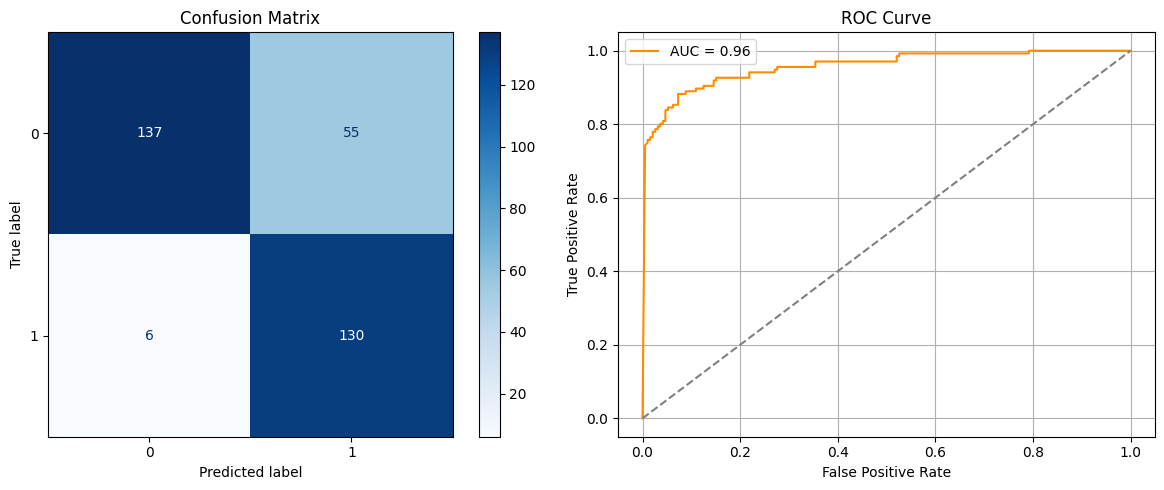
\includegraphics[width=0.9\textwidth]{expt3/nbgauss.png} 
\end{figure}

\begin{verbatim}
# NAIVE BAYES - MULTINOMIAL
evaluate_model("MultinomialNB", MultinomialNB(), X_train, X_test)
\end{verbatim}

\begin{figure}[H]
\centering
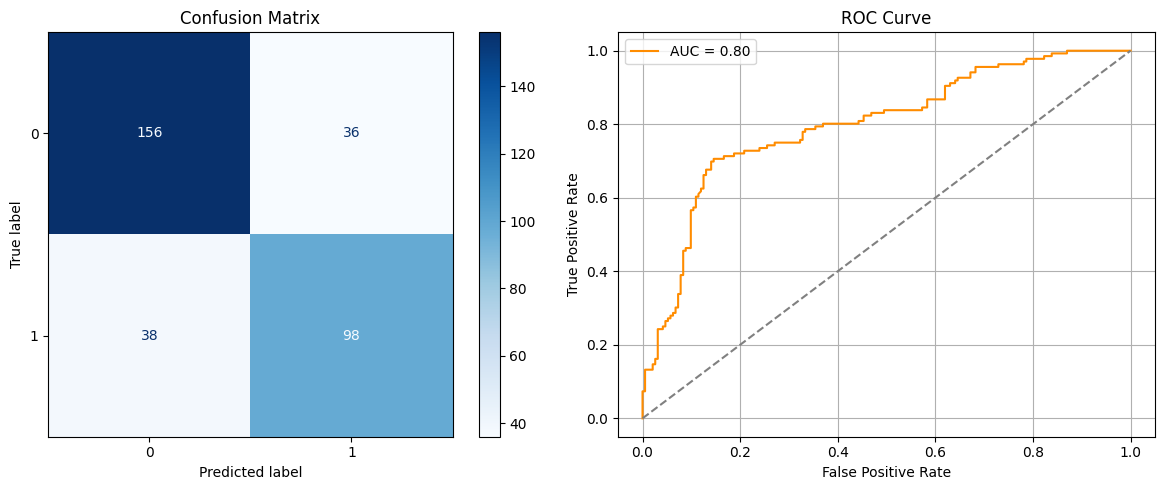
\includegraphics[width=0.9\textwidth]{expt3/nbmulti.png} 
\end{figure}

\begin{verbatim}


# NAIVE BAYES - BERNOULLI
evaluate_model("BernoulliNB", BernoulliNB(), X_train, X_test)
\end{verbatim}

\begin{figure}[H]
\centering
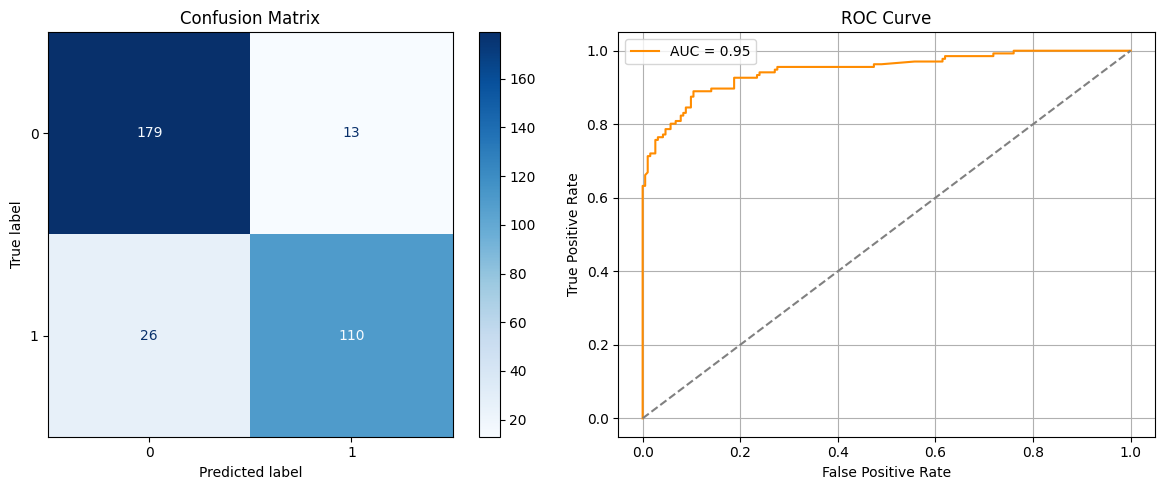
\includegraphics[width=0.9\textwidth]{expt3/nbbern.png} 
\end{figure}

\begin{verbatim}



# K-NEAREST NEIGHBOURS - VARYING K VALUES[1, 3, 5, 7]
for k in [1, 3, 5, 7]:
    evaluate_model(f"KNN (k={k})", KNeighborsClassifier(n_neighbors=k), 
    X_train, X_test)
\end{verbatim}

\begin{figure}[H]
\centering
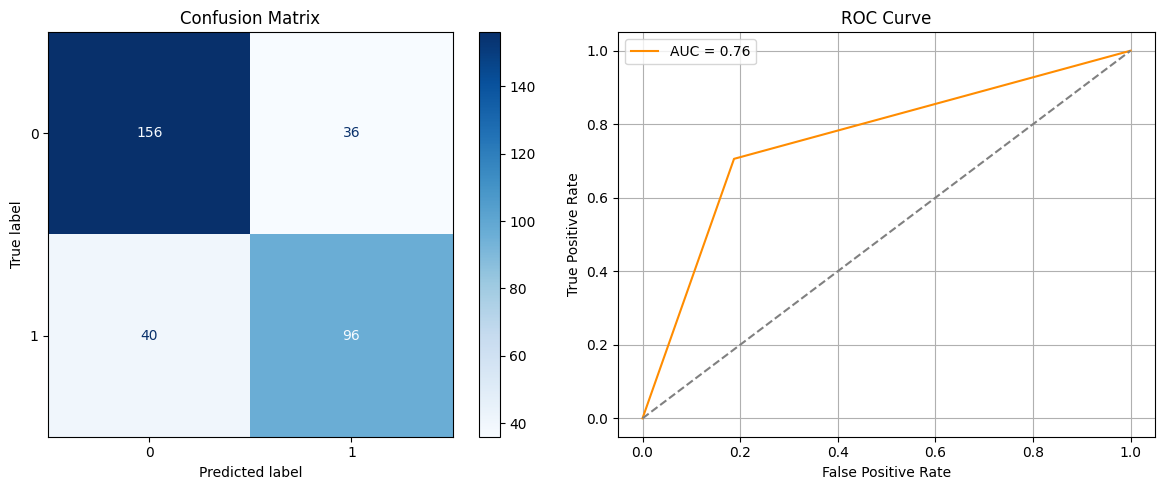
\includegraphics[width=0.8\textwidth]{expt3/knn1.png} 
\caption{k = 1}
\end{figure}

\begin{figure}[H]
\centering
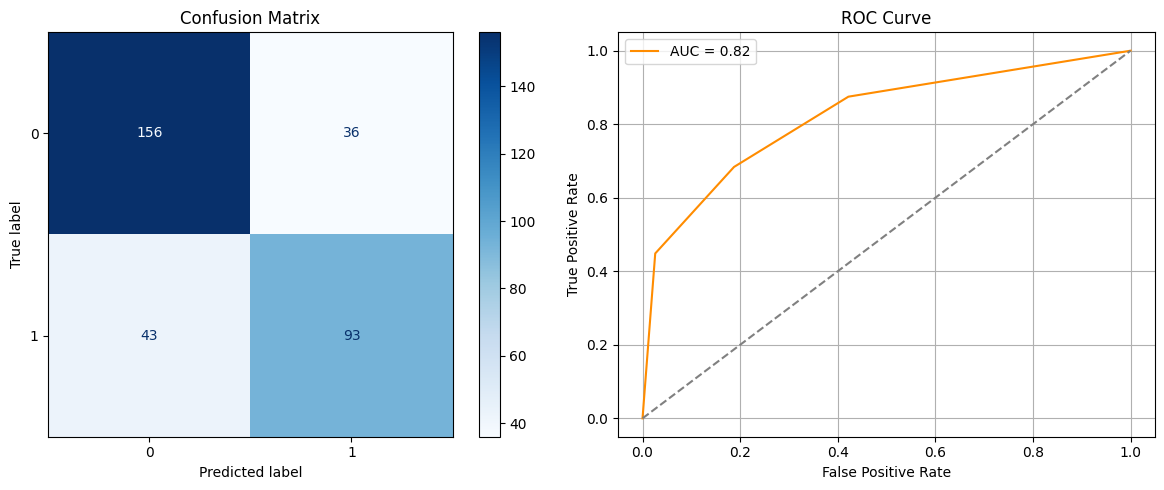
\includegraphics[width=0.8\textwidth]{expt3/knn3.png} 
\caption{k = 3}
\end{figure}

\begin{figure}[H]
\centering
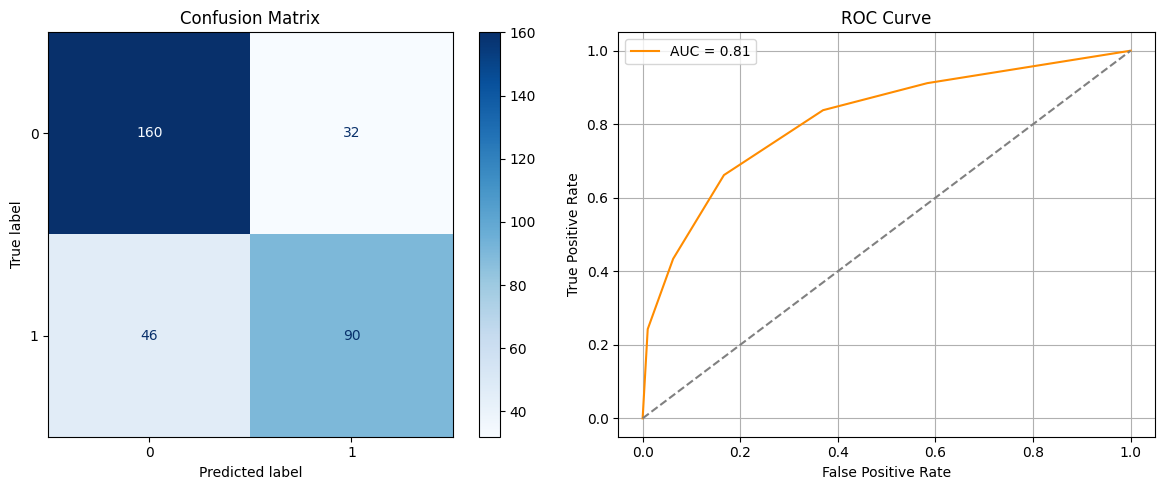
\includegraphics[width=0.8\textwidth]{expt3/knn5.png} 
\caption{k = 5}
\end{figure}

\begin{figure}[H]
\centering
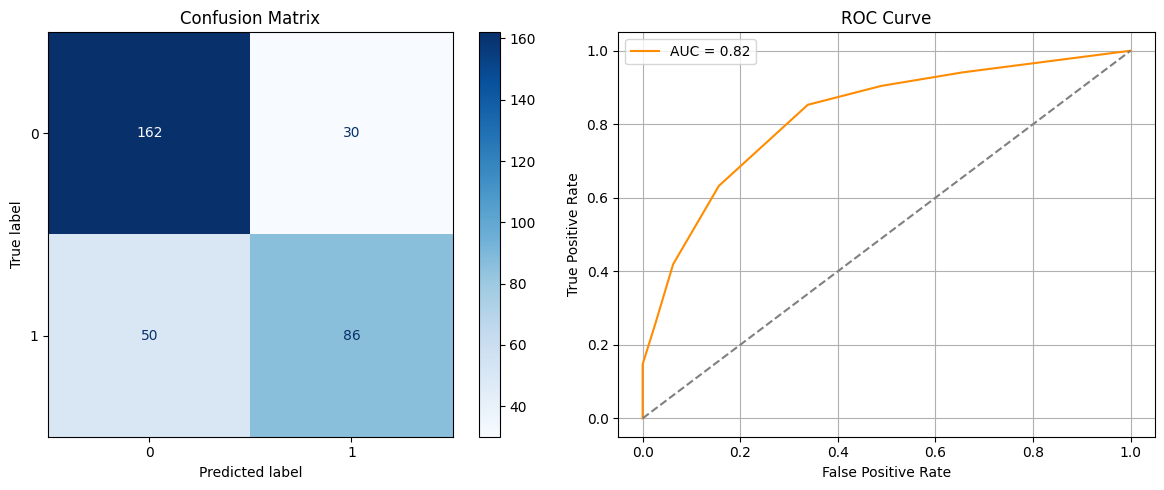
\includegraphics[width=0.8\textwidth]{expt3/knn7.png} 
\caption{k = 7}
\end{figure}

\begin{verbatim}
# K-NEAREST NEIGHBOURS - KDTREE
evaluate_model("KNN (KDTree)", KNeighborsClassifier(algorithm='kd_tree'), 
X_train, X_test)
\end{verbatim}

\begin{figure}[H]
\centering
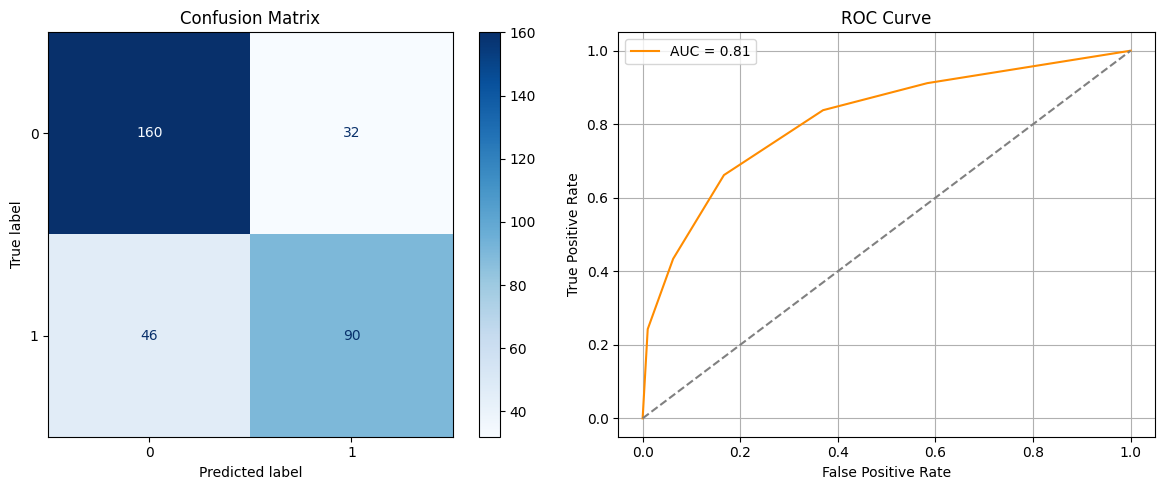
\includegraphics[width=0.8\textwidth]{expt3/kdtree.png} 
\end{figure}

\begin{verbatim}

# K-NEAREST NEIGHBOURS - BALLTREE
evaluate_model("KNN (BallTree)", KNeighborsClassifier(algorithm='ball_tree'), 
X_train, X_test)
\end{verbatim}

\begin{figure}[H]
\centering
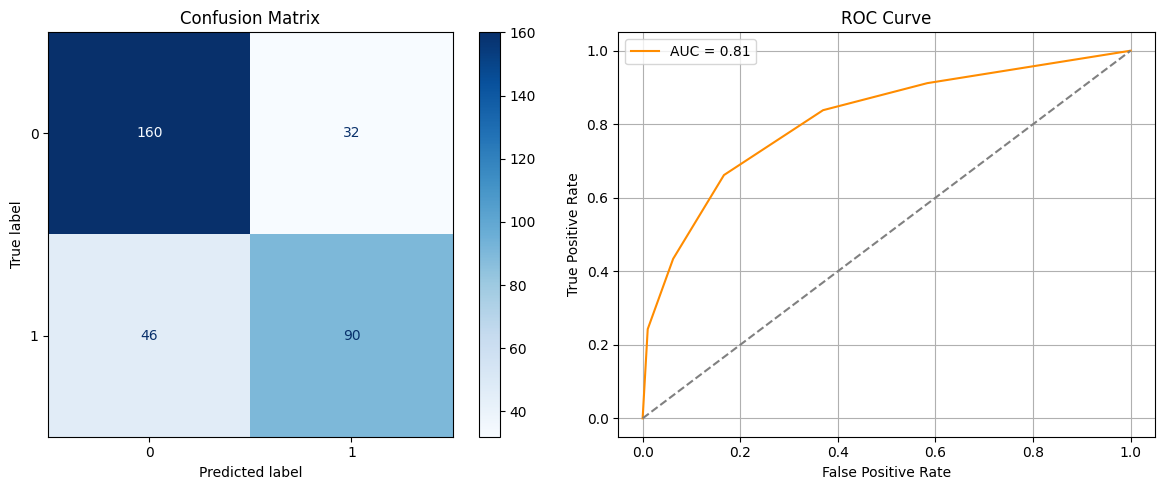
\includegraphics[width=0.7\textwidth]{expt3/balltree.png} 
\end{figure}

\begin{verbatim}
# HYPERPARAMETER TUNING
grid = GridSearchCV(SVC(kernel='linear', probability=False),
{'C': [0.01, 0.1, 1]}, cv=5)
grid.fit(X_train, y_train)
C = grid.best_params_['C']
print("Best C:", C)
\end{verbatim}

\begin{figure}[H]
\centering

\includegraphics[width=0.2\textwidth]{expt3/c.png} 
\end{figure}

\begin{verbatim}

# SUPPORT VECTOR MACHINE - LINEAR
evaluate_model("SVM (Linear)", SVC(kernel='linear', C=C, probability=True), 
X_train, X_test)
\end{verbatim}

\begin{figure}[H]
\centering
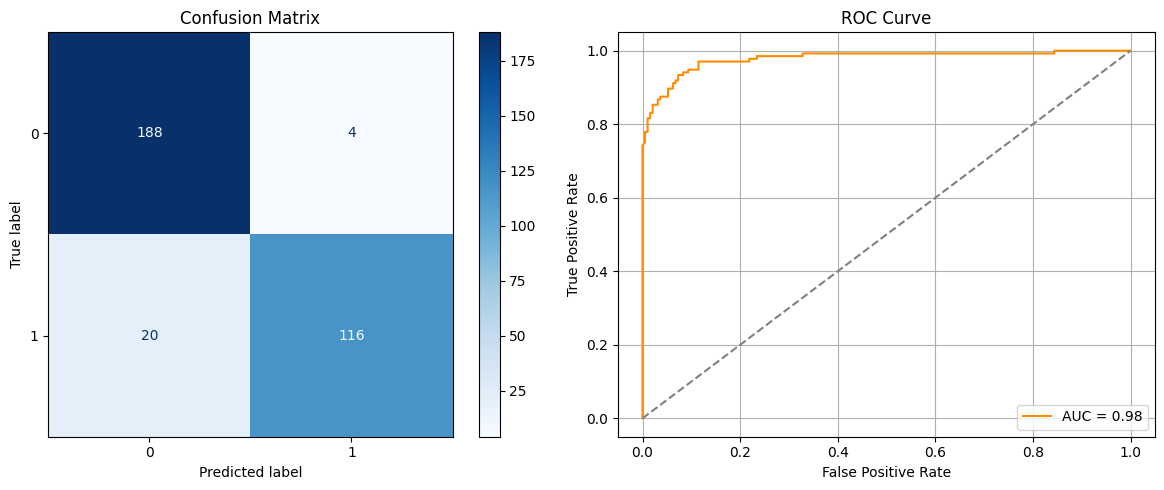
\includegraphics[width=0.8\textwidth]{expt3/linearsvc.png} 
\end{figure}

\begin{verbatim}

# SUPPORT VECTOR MACHINE - POLYNOMIAL
evaluate_model("SVM (Polynomial)", SVC(kernel='poly', C=C, gamma='scale', 
degree=3, probability=True), X_train, X_test)
\end{verbatim}

\begin{figure}[H]
\centering
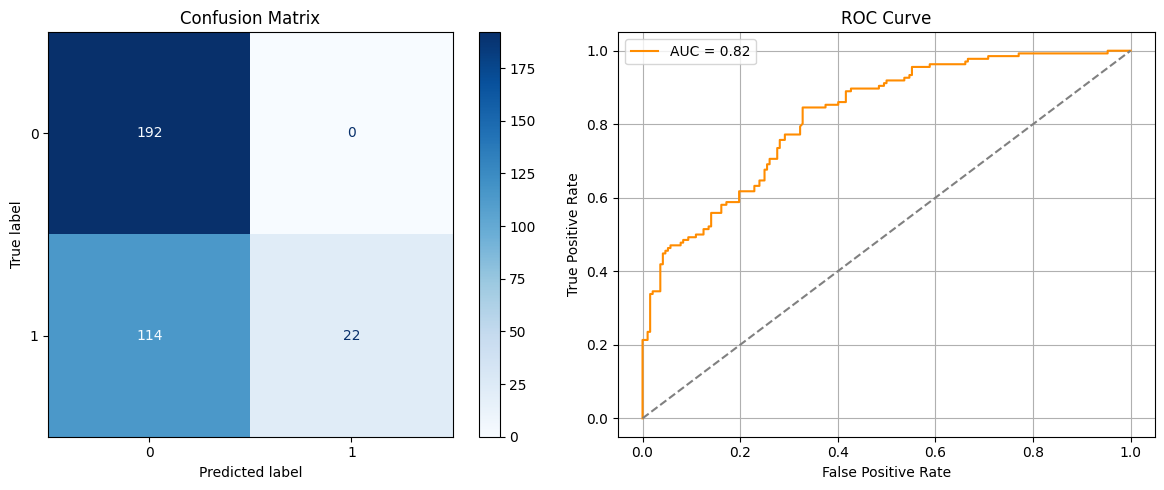
\includegraphics[width=0.8\textwidth]{expt3/polysvc.png} 
\end{figure}

\begin{verbatim}

# SUPPORT VECTOR MACHINE - RBF
evaluate_model("SVM (RBF)", SVC(kernel='rbf', C=C, gamma='auto', probability=True), 
X_train, X_test)
\end{verbatim}

\begin{figure}[H]
\centering
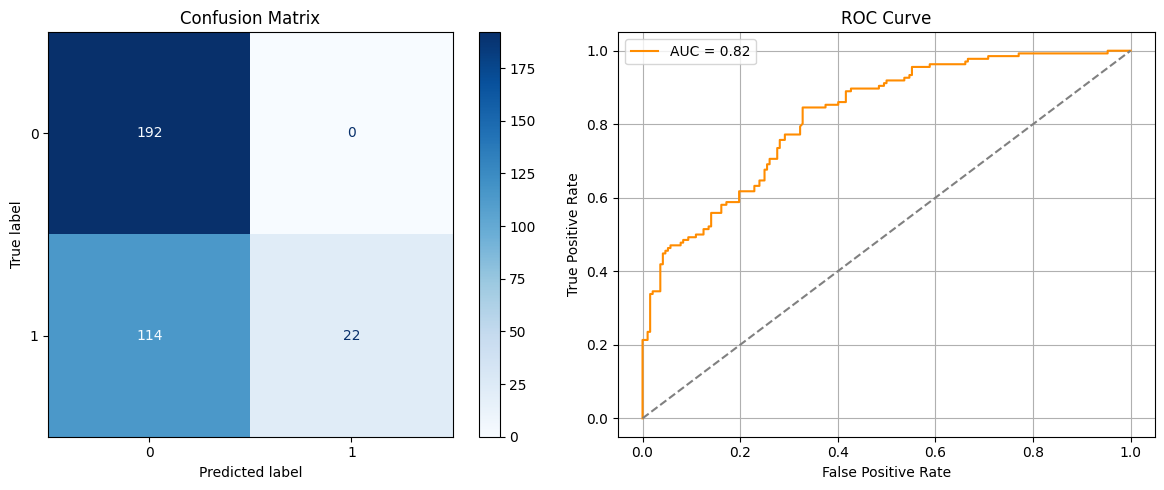
\includegraphics[width=0.8\textwidth]{expt3/polysvc.png} 
\end{figure}

\begin{verbatim}
# SUPPORT VECTOR MACHINE - SIGMOID
evaluate_model("SVM (Sigmoid)", SVC(kernel='sigmoid', C=C, gamma='auto', 
probability=True), X_train, X_test)
\end{verbatim}

\begin{figure}[H]
\centering
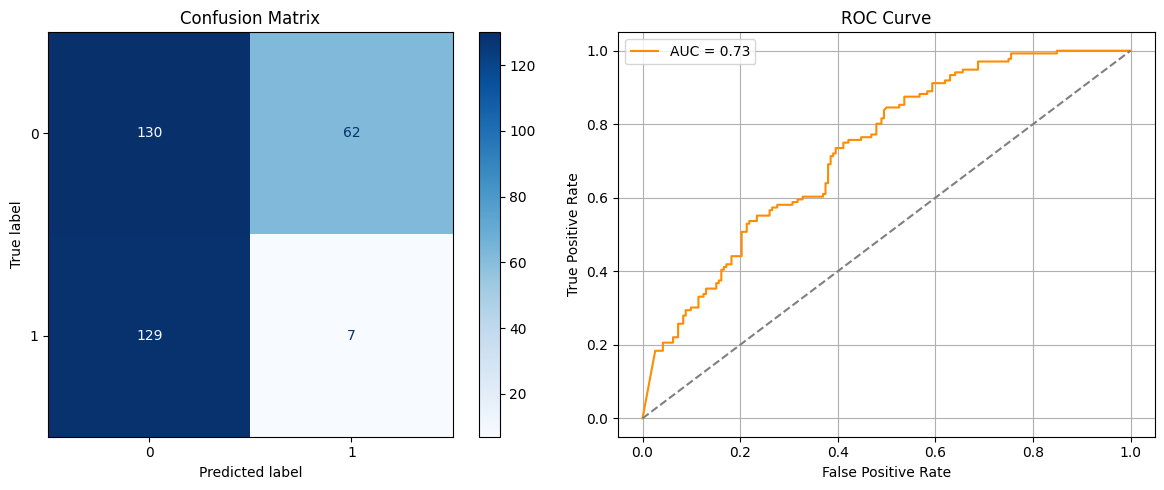
\includegraphics[width=0.8\textwidth]{expt3/sigmoidsvc.png} 
\end{figure}

\begin{verbatim}
# K-FOLD CROSS VALIDATION (K=5)
models = {
    "Naive Bayes": BernoulliNB(),
    "KNN": KNeighborsClassifier(n_neighbors=1),
    "SVM": SVC(kernel='rbf', C=C, gamma='auto', probability=True)
}
kf = KFold(n_splits=5, shuffle=True, random_state=42)
results = {name: [] for name in models}

for fold, (train_idx, test_idx) in enumerate(kf.split(X_encoded), start=1):
    X_train, X_test = X_encoded.iloc[train_idx], X_encoded.iloc[test_idx]
    y_train, y_test = y.iloc[train_idx], y.iloc[test_idx]

    for name, model in models.items():
        model.fit(X_train, y_train)
        acc = model.score(X_test, y_test)
        results[name].append(acc)
        print(f"Fold {fold} - {name} Accuracy: {acc:.4f}")
    print()

print("\nAverage:")
for name, scores in results.items():
    avg_acc = sum(scores) / len(scores)
    print(f"{name}: {avg_acc:.4f}")
\end{verbatim}

\begin{figure}[H]
\centering
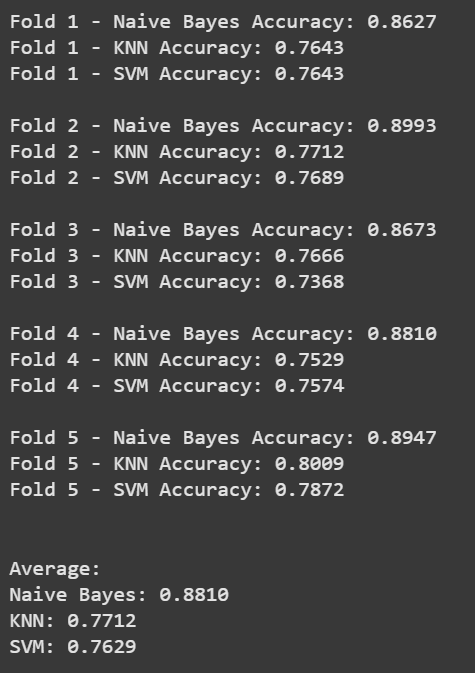
\includegraphics[width=0.6\textwidth]{expt3/kfold.png} 
\end{figure}

\noindent
\section{Comparison Tables:} \\
\vspace{0.5cm}
\textbf{Naïve Bayes Variant Comparison:} \\
\begin{table}[h!]
\centering
\begin{tabular}{|l|c|c|c|c|}
\hline
\textbf{Metric} & \textbf{Gaussian NB} & \textbf{Multinomial NB} & \textbf{Bernoulli NB}\\
\hline
Accuracy & 0.8140 & 0.7744 & 0.8811 \\
Precision & 0.8304 & 0.7677 & 0.8837 \\
Recall & 0.8347 & 0.7665 & 0.8706 \\
F1 Score & 0.8139 & 0.7671 & 0.8756 \\
\hline
\end{tabular}
\caption{Performance Comparison of Naïve Bayes Variants}
\end{table}

\vspace{0.5cm}
\noindent
\textbf{KNN: Varying k Values} \\
\begin{table}[h!]
\centering
\begin{tabular}{|l|c|c|c|c|}
\hline
\textbf{k} & \textbf{Accuracy} & \textbf{Precision} & \textbf{Recall} & \textbf{F1 Score}\\
\hline
1 & 0.7683 & 0.7616 & 0.7592 & 0.7603 \\
3 & 0.7591 & 0.7524 & 0.7482 & 0.7499 \\
5 & 0.7622 & 0.7572 & 0.7475 & 0.7508 \\
7 & 0.7561 & 0.7528 & 0.7381 & 0.7423 \\
\hline
\end{tabular}
\caption{KNN Performance for Different k Values}
\end{table}

\vspace{0.5cm}
\noindent
\textbf{KNN: KDTree vs BallTree} \\
\begin{table}[h!]
\centering
\begin{tabular}{|l|c|c|c|c|}
\hline
\textbf{Metric} & \textbf{KDTree} & \textbf{BallTree}\\
\hline
Accuracy & 0.7622 & 0.7622 \\
Precision & 0.7572 & 0.7572 \\
Recall & 0.7475 & 0.7475 \\
F1 Score & 0.7508 & 0.7508 \\
Training Time(s) & 0.0117 & 0.0089 \\
\hline
\end{tabular}
\caption{KNN Comparison : KDTree vs BallTree}
\end{table}

\vspace{0.5cm}
\noindent
\textbf{SVM Kernel-wise Results} \\
\begin{table}[h!]
\centering
\begin{tabular}{|l|c|c|c|c|}
\hline
\textbf{Kernel} & \textbf{Hyperparameters} & \textbf{Accuracy} & \textbf{F1 Score} & \textbf{Training Time}\\
\hline
Linear & C = 1 & 0.9268 & 0.9231 & 398.0380\\
Polynomial & C = 1, degree = 3, gamma =  & 0.6957 & 0.5476 & 1.1503\\
RBF & C = 1, gamma =  & 0.7872 & 0.7644 & 1.5646\\
Sigmoid & C = 1, gamma =  & 0.4177 & 0.3224 & 0.5035\\
\hline
\end{tabular}
\caption{SVM Performance with Different Kernels and Parameters}
\end{table}

\vspace{1cm}
\noindent
\textbf{K-Fold Cross-Validation Results (K = 5)} \\
\begin{table}[h!]
\centering
\begin{tabular}{|l|c|c|c|c|}
\hline
\textbf{Fold} & \textbf{Naïve Bayes Accuracy} & \textbf{KNN Accuracy} & \textbf{SVM Accuracy}\\
\hline
Fold 1 & 0.8627 & 0.7643 & 0.7643\\
Fold 2 & 0.8993 & 0.7712 & 0.7689\\
Fold 3 & 0.8673 & 0.7666 & 0.7368\\
Fold 4 & 0.8810 & 0.7529 & 0.7574\\
Fold 5 & 0.8947 & 0.8009 & 0.7872\\
\hline
\textbf{Average} & 0.8810 & 0.7712 & 0.7629\\
\hline
\end{tabular}
\caption{Cross-Validation Scores for Each Model}
\end{table}

\vspace{1cm}
\section{Observations and Conclusions}
\begin{itemize}
    \item \textbf{Which classifier had the best average accuracy?}
    \\Naïve Bayes achieved the highest mean accuracy across all classifiers in the 5-fold cross-validation, indicating a strong match between the dataset’s characteristics and the model’s probabilistic assumptions.
    \item \textbf{Which Naïve Bayes variant worked best?}
    \\Of the Naïve Bayes variants tested, Bernoulli Naïve Bayes classifier yielded the best performance, demonstrating superior accuracy compared to Gaussian and Multinomial variants.
    \item \textbf{How did KNN accuracy vary with k and tree type?}
    \\Accuracy decreased as k increased, with the highest accuracy observed at k = 1. The choice of tree type (e.g., KD-Tree vs. Ball Tree) also influenced performance, but the variation was less pronounced compared to changes in k.
    \item \textbf{Which SVM kernel was most effective?}
    \\Among the SVM kernels tested (Linear, Polynomial, RBF, Sigmoid), the Linear kernel achieved the highest accuracy, indicating that the dataset was well-suited to a linear decision boundary.
    \item \textbf{How did hyperparameters influence performance?}
    \\For SVM, the regularization parameter C and the kernel choice were critical, with optimal performance achieved at the tuned C value and the Linear kernel. For KNN, smaller k values improved accuracy, suggesting that the dataset benefits from more localized decision boundaries. 
\end{itemize}

\vspace{3cm}
\section{Learning Outcomes}
\begin{itemize}
    \item Understood and implemented classification algorithms, including Naïve Bayes, KNN, and SVM for binary classification
    \item Applied k-fold cross-validation to obtain reliable performance metrics and reduce model evaluation bias.
    \item Explored the effect of hyperparameters (e.g., k in KNN, C and kernel choice in SVM) on model performance.
    \item Enhanced skills in visualizing results using confusion matrices and ROC curves for model interpretation.
    \item Learned how dataset characteristics influence the suitability of different classifiers.

\end{itemize}

\vspace{1cm}
\noindent
\textbf{GitHub Repository:} \\
\href{https://github.com/vidarshanaa15/ml-expt-3}{https://github.com/vidarshanaa15/ml-expt-3}

\end{document}